\documentclass[a4paper,12pt, headsepline]{scrartcl}

\usepackage[utf8]{inputenc}
\usepackage[T1]{fontenc}
\pagestyle{plain}
\usepackage{lmodern}
\usepackage[english]{babel}
\usepackage[official]{eurosym}
\usepackage{ntheorem}
\newtheorem{hyp}{Hypothesis}
\usepackage{pdfpages}
\usepackage{adjustbox}
\usepackage{footnote}
\usepackage{filecontents}
\usepackage{titling}
\usepackage{csquotes}
\usepackage[objectset = centering]{floatrow}
\usepackage{moreverb}
\usepackage{varioref}
\usepackage{setspace}
\usepackage{graphicx}
\usepackage{tabularx}
\usepackage{dcolumn}
\usepackage{float}
\usepackage{color}
\usepackage{amsmath} 
\usepackage{amsfonts}
\usepackage{float}
\usepackage{mathtools}
\usepackage{relsize}
\usepackage{bm}
\usepackage{dsfont}
\usepackage{algorithm2e}
\usepackage{enumerate}
\usepackage{float}
\usepackage[mathscr]{euscript}
\usepackage[
colorlinks = true,
linkcolor = black,
citecolor = blue 
]{hyperref}

\setlength{\parindent}{0ex} 
\setlength{\parskip}{1ex}


\usepackage[automark]{scrlayer-scrpage}
\setkomafont{pagehead}{\scshape}
\pagestyle{scrheadings}
\ihead{\headmark}
\chead{}
\ohead{}

\cfoot{\pagemark}


\usepackage{csquotes}
\usepackage[
backend=biber,
natbib=true,
language = english,
doi = false, url = false, isbn = false, eprint = false,
style = apa]
{biblatex}
\DeclareLanguageMapping{english}{english-apa}
\addbibresource{literature.bib}

%% Commands %%
\DeclareMathOperator*{\argminA}{arg\,min}
\DeclareMathOperator*{\argmaxA}{arg\,max}
\DeclareMathOperator*{\maxA}{max}
\DeclareMathOperator*{\minA}{min}
%%%%%%%%%%%%%%

% Schrift
\setkomafont{sectioning}{\rmfamily\bfseries\boldmath}

\setcapindent{0em} % kein Einrücken der Caption von Figures und Tabellen
\setcapwidth{0.9\textwidth} % Breite der Caption nur 90% der Textbreite, damit sie sich vom restlichen Text abhebt
\setlength{\abovecaptionskip}{0.2cm} % Abstand der zwischen Bild- und Bildunterschrift
%\renewcommand{\baselinestretch}{1.5}
\numberwithin{equation}{section}
\title{Predicting Award Prices of First Price Sealed Bid Procurement Auctions}
\date{\today}
\author{Fabian Blasch\\[0.4cm]{Supervisor: Dr. Katharina Fenz}}
\begin{document}
\begin{titlingpage}
\maketitle
\end{titlingpage}
\newpage
\tableofcontents
\thispagestyle{empty}
\clearpage
\pagenumbering{arabic} 

\section{Introduction}\label{sec:int}
The importance of public procurement becomes quickly apparent when looking at the sheer volume of contracts that is awarded through public auctions. The authorities of the European Union for example spent around 14\% of their GDP on public procurement in 2017 \citep{GarciaRodriguez2020}. Similar observations can also be made for many states in the U.S. One example of particular importance for this thesis is Colorado. The Colorado Department of Transportation (CDOT), is responsible for procurement of street and bridge construction contracts. As displayed below the budget for transportation is ranked as number four on the largest capital expenditures in the state's budget, after education, health care and human services. Of the approximate 2 billion dollars spent on transportation in 2021, the CDOT awarded \$790 million in contracts, to design, repair and create bridges and highways \citep{CDOTPRes}.

\begin{figure}[H]
	\includegraphics[width = 14	cm]{figures/Colorado_Budget.PNG}
	\caption{Colorado State Operating Budget \citep{ColoradoBudget}}\label{fig:bud}
\end{figure}

Given that the contracts awarded through procurement auctions are such a substantial part of the budget, every potential improvement to the process may greatly increase the efficiency of the tax payers money that is spent. Accordingly, a closer examination of the process including a prediction model for the auctions' award prices may support public procurement agencies like the CDOT with budget planning. Additionally, further analysis of the underlying data in respect to the interactions of particular bidders and the associated effect on award prices is also highly relevant for public procurement agencies. This thesis thus provides an analysis of different models, that predict the award price of an auction given input information available through the bid tabs that are published on the official website of the CDOT. In particular, four different model types with varying preprocessing schedules are compared in terms of their predictive power. Standard linear regression, elastic net regression, random forests and an eXtreme gradient boosting model. To assess, whether, the combination of certain bidders leads to higher award prices, recently discovered post-selection inference methods are utilized \citep{selectiveInference}\\
The remaining paper is structured as follows, first the data extraction process from the PDFs provided on the CDOT's website is described. Then the general process of procurement is outlined, this also entails a concise description of the auction process utilized by the CDOT. The following section covers the methods that are applied, not only in respect to the different models used for prediction but also for the different preprocessing schedules that are applied and the post-selection inference that is used. The thesis concludes with the results for the best predictive model utilizing linear and quadratic loss functions and the results of the analysis of bidder interactions.
\newpage
\section{Data}\label{sec:data}

All the information about the procurement contracts, is obtainable through the bid tab archive on the official website of the Colorado Department of Transportation. The information is provided in PDF documents. In each of those files the following information of the respective auction is provided.

\begin{itemize}
	\item A table listing all submitted bids, including a unique identifier for each of the participating bidders
	\item A contract description
	\item An engineer's estimate
	\item The contract ID
	\item The letting date
	\item Either the amount of time given to complete all the contractual obligations, or a completion due date
	\item The county in which the contract is to be completed in 
\end{itemize}

For illustrative purposes, Figure \ref{fig:bidtab} displays an example of a bid tab, in particular the second page, which contains the vendor ranking as well as the contract description and the remaining information listed above.

\begin{figure}[H]
	\includegraphics[width = 14	cm]{figures/Bid_Tab_exmpl.PNG}
	\caption{Bid Tab Example}\label{fig:bidtab}
\end{figure}

\subsection{Scraping}\label{subsec:scrap}
In order to obtain all the archived bid tabs, the html code of the website was first examined using a google chrome extension called SelectorGadget. This tool allows one to identify html nodes, that website contents are associated with. In the case of the bid tab archive, the html node carrying the links to the individual bid tabs is \enquote{<td a>}. Once this html node is discovered and the consistency across different years in the archive is ensured, the download is easily achieved by looping over the links and downloading the  respective PDFs. The hyperlink extraction was performed utilizing \textit{rvest}, by \citet{rvest}. For the remaining steps in the data extraction process, a distinction will be made for text based information and tabular data.

\subsubsection{Text Based Information}\label{subsubsec:descr}
 The structure of the text based information allows us to filter the individual parts via regular expressions. Especially, for the letting data, the contract ID, and the county this required no further data cleaning steps. Unfortunately, this is not the case for the contract time and the contract description.\\ 
 The contract time was not as straightforward to obtain, since the way it is reported is inconsistent across documents. Most of the time, it is reported as working days until all contractual obligations have to be fulfilled. Seldom, however, the bid tab contains a completion date instead. Accordingly, to achieve consistency across documents all completion dates were converted to contract time. This was achieved by first adding 60 days to the letting date, as this is the number of days that the CDOT reports as the expected time between the letting date and the start of the work on site. Then, the difference in days between the completion date and the starting date were computed. As said difference is only supposed to contain working days the following holidays as well as all weekends were subtracted from the difference between starting date and completion date.
 
 \begin{itemize}
 	\item New Year's Day
 	\item Dr. Martin Luther King, Jr. Day
 	\item President's Day
 	\item Memorial Day
 	\item Juneteenth
 	\item Independence Day
 	\item Labor Day
 	\item Frances Xavier Cabrini Day
 	\item Veterans Day
 	\item Thanksgiving
 	\item Christmas
 \end{itemize}
 
 The computation was executed utilizing the R package \textit{bizdays}, \citet{bizdays}. The package enables the user to generate custom calenders. The difference in starting and completion date was therefore easily calculated by setting up a custom calender with the holidays listed above as well as all Saturdays and Sundays. Then using this calender, the difference between two dates only takes working days into account.
 The only remaining text based information is the contract description. So far, none of the text based information required extensive preprocessing to obtain variables that can be represented in a tabular format. In the case of the contract description this is not the case. In order to convert the contract description into a format that may be represented in a table, the descriptions were first tokenized. Tokenization refers to splitting the input text into single unique words, i.e., splitting the sentences on spaces and removing all forms of punctuation. The result is then a vector of tokens. Said tokens were then scanned for spelling mistakes utilizing the R package \textit{hunspell} \citep{hunspell}. Once the misspelled words were corrected, stop words were removed from the list of tokens. Stop words are words that have no inherent signal associated with their use, examples for such words in the English language would be \enquote{a}, \enquote{is} and \enquote{the}. In natural language processing there is not necessarily one list of stop words, depending on the context different libraries of stop words may be used to remove as much noise as possible from textual data while leaving the signal associated with a series of words in tact. In the case of this thesis, a combination of five different libraries of stop words was used. All of those libraries, \enquote{snowball} , \enquote{stopwords-iso}, 
 \enquote{smart}, \enquote{marimo} and \enquote{nltk} are available through the R package \textit{stopwords}, by \citet{stopwords}. After filtering out the stop words, the remaining words were then stemmed. Stemming refers to the process in which a word is reduced to it's root. This means, that words that carry an identical signal are reduced to the same shortest common substring. Consider the following three words, replacing, replaced, replacement. All those words carry the information that something needs replacement. The language specific circumstances that determine the affixes are not relevant for the information extraction and thus all the aforementioned words are shortened to \enquote{replac} \citet{textminingR}. After stemming, to remove any remaining misspelled words and also for potential removal of unwanted information, all stemmed words were written to an excel file and checked manually. Given that all stop words were already removed and the remaining words were reduced to their stem, this was a very feasible task, resulting in a file with around 2000 words to check. Below we observe the top 40 most frequent words that result from our text mining endeavours.
 
\begin{figure}[H]
	\includegraphics[width = 13.4	cm]{figures/description_words_cloud.pdf}
	\caption{Top 40 Stemmed Description Words}\label{fig:desc}
\end{figure}

\subsubsection{Tabular Data}\label{subsec:tab}

As displayed in Figure \ref{fig:bidtab}, the table in each of the auctions' PDFs contains information on the submitted bids, the bidders' identity and an engineer's estimate. To extract the table containing this information, the package \textit{tabulizer} by \citet{tabulizer} is utilized. This package provides bindings for the Tabula PDF extractor, written in Java. In particular, two functions of the library were combined to write a wrapper for the table extraction. First the function \textit{extract\_tables()} was used to attempt automized table detection and subsequent extraction. Unfortunately, however, there are quite a few cases in which the automatic table detection failed because some auctions only have one or two bidders. The resulting tables that summarize those auctions have very few rows and thus the automatic detection does not recognize them as tables. Accordingly, if the output of \textit{extract\_tables()} is empty, the implemented wrapper calls \textit{extract\_areas()}. This function allows the user to specify an area via the R plot-pane to assess where exactly the table is located. Once the location is passed manually, which was necessary for around 10-15\% of cases, the extraction works as intended. To finally, obtain the tables the wrapper is used to loop over the PDFs.

\subsection{Descriptive Statistics}\label{subsec:desc}
The data that results from the scraping process is based on an auction level. Meaning that each of the 430 auctions that were scraped between 2015 and 2019 represents one row. The final columns are thus:

\begin{itemize}
	\item Contract ID
	\item County
	\item Letting month
	\item Letting year
	\item Contract time
	\item Number of bidders
	\item Engineer's estimate
	\item Award price
	\item 169 binary variables, representing the bidder identities
	\item 652 binary variables, representing pair-wise bidder interaction terms 
	\item 258 binary variables, representing the contract description hit words
\end{itemize}

The interaction terms were generated in order to see, whether, a combination of certain bidders leads to a lower or higher award price. Those terms may also be used to perform unsupervised collusion detection utilizing post-selection inference for $\ell_1$-penalized models. This idea is further outlined in Section \ref{subsec:col}. To obtain a concise overview of the data,  histograms and bar charts of the variables are provided below.

\begin{figure}[H]
	\includegraphics[width = 14	cm]{figures/barplots.pdf}
	\caption{Date, Counties and Number of Firms}\label{fig:barplots}
\end{figure}

We observe, that the sample of auctions in the dataset were held between 2015 and 2019, in which the auction frequency is the highest in January and June. Further we learn, that most contracts are to be completed in El Paso followed by a combination of various counties. In regards to the number of bidders per auction, most of the auctions attract between 1 to 4 bidders, with the maximum being 9 competing firms.

\begin{figure}[H]
	\includegraphics[width = 14	cm]{figures/vend_plots.pdf}
	\caption{Bidders and their Interactions}\label{fig:vendplots}
\end{figure}

The depiction of the top 20 bidders represents the unique identifiers of the firms that submitted the most bids. It is interesting to see that there seem to be a handful of firms that compete in drastically more auctions than others. Additionally, we observe that the two firms that submitted the most bids in the same auctions, compete in slightly more than 10\% of the auctions in the dataset.

\begin{figure}[H]
	\includegraphics[width = 14	cm]{figures/aw_eng_hist.pdf}
	\caption{Award Price and Engineer's Estimate}\label{fig:aweng}
\end{figure}

The last two plots, enable us to gain insights about the distribution of the award price and the engineer's estimate. Both variables are right skewed and to the naked eye the engineer's estimate seems to resemble the distribution of the award price quite well. This is a strong indicator for the engineer's estimate as a predictor. The engineer's estimate is also important as it serves as a benchmark for prediction. Every model that can not beat the engineer's estimate in predicting the award price is not particularly useful, this is further discussed in Section \ref{sec:res}.\\
\newpage
\section{Economic Operationalization}\label{sec:op}

Before formalization, a quick overview of the auction design of the Colorado Department of Transportation is presented. This renders modelling assumptions more comprehensible. The CDOT provides a document on their website that summarizes the entire auction process including all pre-registration processes, that firms have to traverse before they are eligible to submit bids \citep{CDOTRul}.\\
The auction design created by the CDOT is a classical sealed-bid first-price auction, i.e., contracts are advertised for bids online, firms that have been pre-qualified for bidding for a certain contract may submit their bids online or in person. Once a preset date passes a representative of the CDOT opens all submitted bids and announces the lowest bidder, who is awarded the contract. The pre-qualification that was mentioned is of vital importance for this thesis. Given that all firms have to be pre-qualified for bidding, one may utilize bidder identity and bidder interactions when predicting award prices. If there was no pre-qualification, then the auctioneer would not have knowledge of all potential bidders until no more bids are to be received. At this point there is also no need for a prediction of the award price. Besides a pre-qualification process, the CDOT also implements a reserve price. Every project is assigned an engineer, who is responsible to calculate an engineer's estimate of the cost of completion. Should the lowest bid that was submitted exceed the engineer's estimate by more than 10\%, then the lowest bidder is only awarded the contract if a secondary assessment of the CDOT ends with the conclusion that the lowest apparent bid is indeed a reasonable price for execution of the contractual obligations. This secondary process to bypass the initial reserve price was necessary for 17\% of the auctions in the dataset that is used in this thesis. In regards to the frequency of bid rejection, for our modelling assumption it is important to know that the secondary assessment process very rarely results in a rejection of the lowest apparent bid \citep{CDOTRul}. 

\subsection{First Price Sealed Bid Auctions}\label{subsec:fpsba}

For the applied nature of this thesis a formalization of the auction process in not a necessary prerequisite 
for a good prediction model, however, a sound understanding of all the economic agents at play might yield insights into the potential benefit of a prediction model for participating firms and it may also provide us with expectations for the post-selection inference that is explored in Section \ref{subsubsec:psi}. Given that this chapter is not strictly necessary for the reader to understand the main findings of this thesis a basic understanding of game theory is assumed. The interested reader is referred to, \citet{tadelis12}, who provides sound definitions and explanations of all the required concepts.\\
The description of bidding in the first-price sealed-bid procurement auction (FPSBPA) is denoted in accordance with \citet{milgrom82} and \citet{HandbookIndustrialOrga}. For the following formalization let uppercase letters represent random variables and their lowercase counterpart a single realisation. Consider an auction environment with $n$ potential bidding firms, all of them submit bids in hopes to procure a contract from the auctioneer. Each of those firms, which are indexed by $i$ observe a real valued signal $x_i$. One can think of $X_i$ as private information that each firm has about their own cost structure and other private information that a bidder can posses, that influences the value of a contract to a firm. Further, let $V$ represent the characteristics that determine the value of the contract to the firms, that are common knowledge among competing bidders. For illustrative purposes, consider an auction for a contract that involves the repair of a street that leads up a mountain. The information that can be extracted from the contract description is common knowledge, i.e., it influences the value of the contract of every firm. Every bidder is aware that a street, which is steep is more cost intensive to repair. When modelling the bidders behaviour we assume that this is common knowledge, such common values are represented by $V$. In the auction modelling literature, a distinction is made between an auction environment of private values, i.e., each firm knows their own valuation and is only uncertain about how other firms value the contract. The counterpart to this auction environment is one of pure common values. In this case all bidders have the same common value, however, prior to the execution of the contractual obligations they have no accurate ex ante estimate of the value that may be extracted from completing this contract. This common value paradigm is important when modelling because, given that firms have common metrics that make contracts more or less attractive, makes the private information that firms may posses relevant for rival bidders and will thus influence the ex post value once all bids are revealed. To continue the formalization of the auction environment, let firm $i's$ payoff be represented by $U_i = u_i(V, X_i, X_{-i})$, where $X_{-i}$ represents the private information possessed by firm $i's$ rivals. Most of the time it is assumed that firms are risk neutral, i.e., expected utility of profit is simply equal to the expectation of a linear function of capital gained, and maximizing it is equivalent to maximizing expected profit itself. The payoff or the value of a contract to a firm may then be defined as the expectation of $U_i$ given the private information of firm $i$, i.e., $\mathbb{E}(U_i|X_i = x_i, X_{-i} = x_{-i})$. It is important to point out, that in a common values environment the distribution of V conditional on $x_{i}$ is dependent on the realization of $X_{-i}$. This means that from the perspective of firm $i$, other firms may have private information about characteristics of a contract that influence it's value to all competing firms and thus also the value in the eyes of firm $i$. Accordingly, let the bidding strategy be a mapping $\beta: X_i \rightarrow \mathbb{R}^+$, that maps the private information of firm $i$ (cost structure, private knowledge about a contract obtained through on site inspections, ...) into the non-negative real numbers. To ensure that this function is invertible, in the literature it is usually assumed that $\beta$ is a bijection that is strictly increasing in the signal $X_i$. Again, assuming that $X_i$ represents the cost structure of firm $i$ and other private information, a ceteris paribus decrease in costs is then associated with a decrease in the price of submitted bids. Now that the basic formalities of the auction environment have been set, we may consider the \enquote{winner's curse}, which assumes the event of winning an auction as an informative event in respect to the value of the contract. The idea is that a firm that manages to procure a contract through an auction must be the lowest bidder, and this also means that no other firm was willing to execute the contractual obligations for the same price. More formally, assume that the realization $v$ is unknown and carries a significant common component. Additionally, we may assume that all firms have varying amounts of private information about the contract. They are aware that other firms have private information but they are uncertain about other firms' valuations of the contract. Further, to simplify the model we assume that the signals $x_i$ are drawn from a common distribution $F$ and that the value of the contract is mainly determined by the common component of bidders' valuations, i.e, w.l.o.g for firm 1, the ex ante valuation of the contract is equal to:
\[
v_1(x_1) = \mathbb{E}[V|X_1 = x_1]  = \int vf_{V|X_1}(v|x_1)dv.
\]
 Then in equilibrium, assuming that the bidding function is increasing in the cost realization, the winner is the firm with the lowest cost draw from the distribution but also influenced by the firms private information about the contract. Formally, in the literature this is formalized by stating that the lowest bid is announced by the firm that incurs the lowest signal \citep{HandbookIndustrialOrga}. This intuitively makes sense as the signal is defined on the real numbers and the lowest signal will thus be identical to the lowest contract execution costs and consequently the highest profit to be made. By Jensen's inequality, given that the maximum is a convex function, 
\[
\mathbb{E}[\text{max}\{V_i|v\}] \leq \text{max}\{{\mathbb{E}[V_i|v]}\} = v.
\] 
This represents the winner's curse as the firm with the lowest signal submits the lowest bid. Further as \citet{milgrom82} state, w.l.o.g, for firm 1 this means:
\[
\mathbb{E}[V|X_1 = x, Y_1 > x] < \mathbb{E}[V, X_1 = x].
\]
Where $Y_1$ is the firm with the lowest signal among firm 1's rivals. We thus find that the bidder that incurs the lowest signal associated with the completion of all contractual obligations and therefore the highest potential profit to be extracted from the procurement of the contract should bid less than the firm's ex ante estimate of $V_1$, simply because the assignment of the contract to the firm as the lowest bidder is an informative event. Especially for firms, that are not as established and might have difficulties to obtain the expertise to properly assess the difficulties associated with completion of a contractual agreement will suffer more severely from the winner's curse. This is relevant for this thesis as an award price prediction that gives a reasonable estimate for the costs associated with the completion of a contract will change the informational asymmetries and thus also lessen the severity of the winner's curse, should the award price prediction be shared with the bidders \citep{GarciaRodriguez2020}.\\
Now that we have discovered another potential beneficiary of a award price prediction model, we may assess the strategic bidding behaviour of firms. To further simplify the strategic behaviour we may assume that firms signal realisations $x_i$ are drawn from a common distribution, i.e., the value associated with a contract $(V, X_1, ..., X_n)$ are governed by some joint distribution denoted by F. Further, we may assume that the number of firms that submit bids is common knowledge and that the reserve price is not binding. Essentially, this means that the firms believe that bidding above the 110\% threshold will not lead to a reissue of the contract but to a contract award in the secondary process previously described. Given that this game is symmetric, we may again focus on firm 1, w.l.o.g. The firm then aims to maximize its expected profit, i.e.,
\[
\argmaxA_b \text{ } (b - x)\{1 - F[\beta^{-1}(b)]\}^{n-1}.
\]
Where $(b - x)$ is the profit that the firm expects if it were to win the contract and the remaining term is the probability that all other competing bidders incur a higher signal realization associated with the execution of the contractual obligation, and thus submit higher bids. Accordingly, by the previously mentioned assumption of the strictly increasing function $\beta$, the lowest signal leads to the lowest bid. From the maximization problem, we obtain the following FOC:
\begin{gather*}
\{1-F[\beta^{-1}(b)]\}^{n-1} + (b - x)(n - 		1)\{1-F[\beta^{-1}(b)]\}^{n-2}\frac{d\beta^{-1}}{db}\{(-1)f[\beta^{-1}(b)]\} \overset{!}{=} 0\\
	\iff \frac{\{1-F[\beta^{-1}(b)]\}^{n-1}}{\{1-F[\beta^{-1}(b)]\}^{n-2}} = (b - x)(n - 1)f[\beta^{-1}(b)]\frac{d\beta^{-1}}{db}\\
	\iff 1-F[\beta^{-1}(b)] = (b - x)(n - 1)f[\beta^{-1}(b)]\frac{d\beta^{-1}}{db}
\end{gather*}
Knowing that in the bayesian NE, $\beta^{-1}(b) = x$ and $\frac{d\beta^{-1}(b)}{db} = \frac{1}{\beta'(x)}$, we then find:
\begin{gather*}
	\beta'(x) = \frac{[\beta(x) - x](n - 1)f(x)}{1-F(x)}
\end{gather*}
This is a differential equation that modern computer algebra systems like mathematica can easily solve to obtain the bayesian NE bid function \citep{mathematica}.
\[
\beta(x) = x + \frac{\int_x^\infty [1 - F(t)]^{(n-1)}dt}{[1-F(x)]^{(n-1)}}
\]
We thus learn that the bid resulting from the cost structure of the firm is a surcharge added to the realization of $X$. Again, we may interpret this as the private information of firm $i$ on the cost of completion of the contractual obligations, e.g., information about the firms cost structure, information about execution costs obtained from on-site inspections, etc. Further, we observe that the surcharge depends on the number of firms in an auction and the joint distribution $F$. We have to keep in mind, however, that this simple result is based on quite restrictive assumptions. Especially, the risk neutrality of firms is not particularly realistic. Nonetheless, given those simplifying assumptions, the results displayed in section \ref{sec:res} will show, whether, the derived economic intuition of firms behaviour is observable in the data.
\newpage
\section{Methods}\label{sec:meth}

This section contains precise descriptions of the methods used to generate the results presented in section \ref{sec:res}.

\subsection{Elastic Nets}\label{subsec:net}

When the number of features in a dataset is significantly larger than the number of observations, elastic net regularization offers a solution to fit linear models using a convex combination of the lasso and ridge penalty. Further the regularization, may be used to better optimize the bias variance trade-off when compared to standard linear regression.\\
The description of the elastic net regularization is denoted in accordance with the seminal paper by \citet{hastie03}. Assume that a dataset has $n$ observations and $p$ explanatory variables. As it is the case with the auction dataset, the number of explanatory variables may greatly exceed the number of observations, i.e., $p >> n$. Let $\mathbf{y} = (y_1, ...., y_n)^T$ be the response variable and $\mathbf{X} = [x_1|...|x_p]$ the model matrix, containing the hot encoded explanatory variables. This means that all factor variables have to be converted to individual dummy variables for each level. Subsequently, each column in the model matrix is then centered and standardized. This ensures that the regularization is consistent across variables, since the regularization process is not scale invariant. For any combination of non-negative $\lambda_1$ and $\lambda_2$, \citet{hastie03}, define the elastic net criterion as,
\[
L(\lambda_1, \lambda_2, \bm{\beta}) = |\mathbf{y} - \mathbf{X}\bm{\beta}|^2 +\lambda_2|\bm{\beta}|^2 +\lambda_2|\bm{\beta}|_1, 
\]
where $|\bm{\beta}|^2$ represents the $\ell_2$ norm of the coefficient vector $\bm{\beta}$, i.e., 
\[
|\bm{\beta}|^2 = \mathlarger{\sum}\limits_{i = 1}^{p}\bm{\beta}_i^2
\]
and $|\bm{\beta}|_1$ is equivalent to the $\ell_1$ norm, i.e.,  
\[
|\bm{\beta}|_1 = \mathlarger{\sum}\limits_{i = 1}^{p}|\bm{\beta}_i|.
\]
The elastic net estimator $\bm{\hat{\beta}}$ results from the following minimization problem,
\[
\bm{\hat{\beta}} = \argminA_{\bm{\beta}} L(\lambda_1, \lambda_2, \bm{\beta}).
\]
Alternatively, the elastic net penalized regression may also be written as a constrained optimization problem of the least square estimator. Let $\alpha = \frac{\lambda_2}{\lambda_2 + \lambda_1}$, then for some fixed $t$, 
\[
\bm{\hat{\beta}} = \argminA_{\bm{\beta}} |\mathbf{y} - \mathbf{X}\bm{\beta}|^2,
\]
subject to,
\[
(1 - \alpha)|\bm{\beta}|_1 + \alpha|\bm{\beta}|^2 \leq t.
\]
The constraint thus encompasses a convex combination of the lasso penalty and the ridge penalty. Accordingly, both ridge and lasso regression are a special cases of an elastic net, where $\alpha = 1$ results in ridge regression and $\alpha = 0$ leaves us with the $\ell_1$ penalized lasso regression estimator, initially presented by \citet{tibshirani96}. In regards to model selection, lasso regression is particularly powerful as it does not shrink candidate variables close to zero, which is the case when utilizing the ridge penalty. In the case of $\ell_1$ penalized regression, the obtained $\bm{\hat{\beta}}$ carries only non-zero components for the variables that were deemed important enough in the cross-validation process used to determine the optimal value of the shrinkage parameter $t$, assuming $\alpha = 0$. This is troublesome for the frequentist statistician, as it implies that the coefficient vector $\bm{\hat{\beta}}$ itself is random \citep{Lee2016}. The severity of the implications for frequentist inference is outlined in \citet{benjamini05} and \citet{benjamini09}.

\subsubsection{Post-Selection Inference for $\ell_1$-Penalized Models}\label{subsubsec:psi}
Having discovered the randomness introduced by shrinkage to exactly zero of some elements in the coefficient vector $\bm{\hat{\beta}}$, it is important to develop a sound understanding of the source of randomness. The randomness introduced by variable selection is one of choice and not inherent to the parameter value itself. Denoted in accordance with \citet{Lee2016}, again we assume $p$ explanatory variables. Further, let $M\subset\{1, ..., p\}$ be the subset of covariates which estimate $\beta_j^M$ has not been set to zero given the optimal choice of the regularization parameter $t$. Formally we may write,
\[
\{\beta_j^M: M\subset\{1, ..., p\}, j \in M\}.
\]
Given $t > 0$, we will only draw inference from the coefficients $\hat\beta_j^{\hat M}$, i.e., the estimates chosen by the applied $\ell_1$ regularization process, $\{\hat M: \hat\beta_j \neq 0\}$. Thus the randomness is introduced by the choice of $\hat M$. Now that the problem inherent with the choice of $\hat M$ is established, we may consider a solution to draw valid inference as presented by \citet{Lee2016}. Suppose we want to create a confidence interval $C_j^{\hat M}$ for a parameter $\hat\beta_j^{\hat M}$, then fixing $\alpha$ as the desired type I error we want the confidence interval to fulfill:
\[
\mathbb{P}(\beta_j^{\hat M} \in C_j^{\hat M}) \leq 1 - \alpha.
\]
Unfortunately, this is obviously undefined for all $j \notin \hat M$. Accordingly, to resolve this issue \citet{Lee2016} rely conditional convergence. Since we construct an interval for $\hat\beta_j^{\hat M}$ iff $\hat M$ is selected, we may condition on this event. Thus we obtain,
\[
\mathbb{P}(\beta_j^{\hat M} \in C_j^{\hat M}| \hat M = M) \leq 1 - \alpha.
\]
In order to obtain the interval mentioned above, \citet{Lee2016} study the conditional distribution,
\[
\bm{\eta_M^Ty}|\{\hat M = M\},
\]
which allows, in theory, to draw inference from parameters of the more general form $\bm{\eta_M^T\mu}$. To then characterize the event, $\{\hat M = M\}$ for lasso regression the resulting event is a union of polyhedra, i.e., $\{\hat M = M, \hat s_M = s_M\}$, that conditions on the specified explanatory variables as well as the signs of the selected covariates. Formally this may be stated as,
\[
\bm{y} \in \mathbb{R}^n: A(M, s_M)\bm{y} \leq \bm{b}(M, s_M)
\]
and hence when conditioning on the sign as well as the selected variables, it is sufficient to study,
\[
\bm{\eta^Ty}|\{A\bm{y} \leq \bm{b}\}.
\]
\citet{Lee2016}, elegantly derive that the resulting conditional distribution is a univariate truncated Gaussian. Subsequently, they use this result to present a test statistic that may be utilized to draw inference about the significance of the parameter estimates $\hat\beta_j^{\hat M}$. A description of this derivation is beyond the scope of this thesis, the interested reader is referred to \citet{Lee2016} and \citet{tib2016}. Where the latter provides an extension to the results of \citet{Lee2016}, to generalized $\ell_1$ penalized linear models and further also provides the implementation in an R package called \textit{selectiveInference}, by \citet{selectiveInference}.

\subsection{Ensemble Methods}\label{subsec:ens}
Ensemble methods encompass the combination of simple learning algorithms to achieve superior results in regard to predictive power. For this thesis tree-based methods are of particular importance. For the sake of simplicity, we may only distinguish between two methods of combining individual trees. Bagging and boosting, the former revolves around bootstrap aggregation, which might be a more familiar term to some readers, that have not been exposed to a lot of machine learning literature. Bootstrap aggregation aims to reduce the variance of prediction, by sampling with replacement from all observations, to then apply some simple learning algorithm like a regression tree. In the end the resulting prediction is a constant derived from the individual learners, most of the times said constant is the arithmetic mean. In contrast, boosting aims to improve the predictive power of simple learners like regression trees by sequentially improving the error of the previously fit tree. This chapter gives a concise overview of regression trees as the base learners, random forest which utilizes bagging and eXtreme Gradient Boosting which as the name suggests is a special boosting technique discovered by \citet{chen2016}. The formalization of those methods is denoted in accordance with \citet{hastie09} for regression trees and random forest. For eXtreme gradient boosting the notation is heavily inspired by the seminal paper by \citet{chen2016}. As previously, it is assumed that the reader is familiar with basic terminology, should some terms be unfamiliar, the reader is referred to \citet{James2013} and \citet{hastie09}. Where the former provides a very informal and easy to understand approach, while the latter is more formally motivated.
\subsubsection{Regression Trees}\label{subsubsec:trees}
The description simple learner could not be more fitting than in the case of a regression tree. In essence the idea may be described in a single sentence. A regression tree finds recursive binary partitions in the space spanned by the explanatory variables that optimizes some metric used to judge the best variable as well as the best available value to form a partition. More formally, again let $p$ represent the number of explanatory variables and $n$ the number of observations, i.e., $i = 1, 2, ..., n$ and $x_i = (x_{i1}, ..., x_{ip})$. Further, let there be M regions $R_i$, each formed by a split in the data. Additionally, suppose that we model the response variable $y$ as a constant $c_m$ in each region, i.e.,
\[
f(x) = \mathlarger{\sum}\limits_{m = 1}^{M} c_m \mathds{1}_{\{x \text{ } \in \text{ } R_m\}}.
\]
If we choose to minimize the sum of squares, 
\[
\mathlarger{\sum}\limits_{i = 1}^{n}(y_i - f(x_i))^2,
\]
the optimal $\hat c_m$ is the arithmetic mean of the observations in partition $R_i$ \citep{hastie09}. A proof for this statement would be identical to deriving the optimal value of the intercept in a linear model that is only made up of one constant. So far, we have determined how to optimally represent the observations grouped in a partition $R_i$ by a single constant. However, we still need to determine how to choose the optimal splitting variable $x_j$ as well as the optimal splitting point $s$. Suppose that at each node, we consider all possible variables $p$ that may generate the best pair of resulting half planes,
\[
R_1(j, s) = \{X|X_j \leq s\} \text{ and } R_2(j, s) = \{X|X_j > s\}.
\]
We aim to choose the splitting variable $j$ and the corresponding splitting point $s$ such that,
\[
\minA_{j, s}\mathlarger{[} \minA_{c_1} \mathlarger{\sum}\limits_{x_i \in R_1(j, s)} (y_i - c_1)^2 + \minA_{c_2} \mathlarger{\sum}\limits_{x_i \in R_2(j, s)} (y_i - c_2)^2 \mathlarger{]}.
\]
Note that that it is infeasible to choose those sequential partitions that optimize the sum of squares simultaneously for all possible splits. Accordingly, the optimization process is greedy in a sense that it is memoryless and only considers the current available splits given all splits that have occurred beforehand. To a degree this is quite unsettling as it does not guarantee that the recursive partitioning will lead to a global minimum in RSS. This is also where ensemble algorithms may make quite a difference, as we will discover at a later stage. Coming back to the greedy minimization, we have previously discovered that the inner minimum in regards to the constant that represent the observations in $R_1$ and $R_2$ are optimally represented by the arithmetic mean. The outer minimum in respect to $j$ and $s$ may be discovered by  finding the best splitting point $s$ for every candidate variable $j$ to then assess which combination $(j, s)$ leads to the minimization in RSS. This process may then be repeated in the resulting half-planes. If we were to consider trees as a stand alone learner, at this point we would have to think about how we choose the complexity of the tree. However, as in this thesis the depth of a tree is a hyper parameter chosen via cross validation we may skip this part. The interested reader is referred to \citet{hastie09}. Shortly summarized, fixing some threshold for the minimum decrease in RSS to warrant an additional split is not optimal as a seemingly bad split at the current node  might lead to a significant decrease in RSS at a later split. Accordingly, what is usually applied to determine the optimal tree complexity is cost-complexity pruning. In essence this means the tree is grown until some minimum node size is reached and then the tree is \enquote{cut down} backwards starting from the terminal nodes.

\subsubsection{Random Forest}\label{subsubsec:rf}
As previously mentioned random forests utilize bootstrap aggregation to improve the predictive performance of many noisy but unbiased learners. This is achieved by reducing the variance of the individual simple learning algorithm. The presented regression trees are well suited for this, as they may capture complex non-linear relationships in the data and given that they are grown sufficiently deep, they exhibit low bias. For the sake of simplicity, the notation is slightly changed. Let the dataset be defined as $\mathcal{D}\{\{\bm x_i, y_i\}\}$, with $i = 1, ..., n$, $\bm x_i \in \mathbb{R}^p$ and $y_i \in \mathbb{R}$. The algorithm used to fit a random forest may be concisely described following \citet{hastie09}:

\RestyleAlgo{ruled}

%% This is needed if you want to add comments in
%% your algorithm with \Comment
\SetKwComment{Comment}{/* }{ */}
% A distance matrix based on pairwise euclidean distance $\mathbf{D} \coloneqq Dist(G_i, G_j)\text{ }\forall\text{ }i, j$,\\
{\centering
\begin{minipage}{.9\linewidth}
	\begin{algorithm}[H]
		\caption{\textit{Random Forest}}\label{alg:one}
		\KwData{$b = 1, 2, ..., B$ bootstrap samples drawn with replacement from the training data, $p$ the number of explanatory variables, $m$ the number of variables sampled for each split, $n_{min}$ the minmum node size and the maximum depth $d_{max}$.}
		\begin{enumerate}
			\item For each bootstrap sample b, grow a regression tree $T_b$ utilizing the bagged data, by recursively repeating the following steps, until the minimum node size $n_{min}$ or the maximum depth $d_{max}$ is reached.
			\begin{enumerate}[i.]
				\item Randomly sample $m$ explanatory variables from the $p$ available candidates.
				\item Find the best split point $s$ for each of the sampled variables $m$.
				\item Choose the best split available.
			\end{enumerate}
			\item Return the ensemble of trees $\{T_b\}_1^B$
		\end{enumerate}
	\end{algorithm}
\end{minipage}
\par
}
To predict the response of a new observation, we simply average over the trees in our forest, i.e,
\[
\hat f_{rf}(\bm x_i) = \frac{1}{B} \mathlarger{\sum}\limits_{b = 1}^B T_B(\bm x_i).
\]
 By linearity of the expectation operator, given that each tree generated in bootstrap aggregation is identically distributed, we find that the expectation of the average of an ensemble of trees is identical to any of the individual trees. Put differently, the bias of any single tree is identical to the bias of the bagged ensemble and thus the only way of improving the predictive accuracy is via a reduction in variance.
 To gain further insights into the workings of a random forest we may benefit from examining the variance of the $B$ random variables $T_b$ that represent the trees in our forest. Note that said trees are identically distributed but not necessarily independent. Let the variance of $T_b$ be represented by $\sigma^2$ and further let the positive pairwise correlation be represented by $\rho$. Accordingly, the prediction that we obtain by averaging over all trees in the forest exhibits the variance: 
 \[
 \mathbb{V}\text{ar}(\hat f_{rf}) = \mathbb{V}\text{ar} \left[ \frac{1}{B} \mathlarger{\sum}\limits_{b = 1}^B T_B(\bm x_i) \right] = \frac{1}{B^2} \mathbb{V}\text{ar} \left[ \mathlarger{\sum}\limits_{b = 1}^B T_B(\bm x_i) \right] = \frac{1}{B^2} \mathlarger{\sum}\limits_{k = 1}^B \mathlarger{\sum}\limits_{j = 1}^B \mathbb{C}\text{ov} \left[T_k, T_j \right].
 \]
Now, given that in the double sum there are $B^2$ summands and we know that B of those are just $\mathbb{C}\text{ov}\left[T_k, T_k \right] = \mathbb{V}ar\left[T_k\right] = \sigma^2$, we are left with $B^2 - B$ terms for all cases $k \neq j$, and we thus find,
\[
\frac{1}{B^2} \mathlarger{\sum}\limits_{k = 1}^B \mathlarger{\sum}\limits_{j = 1}^B \mathbb{C}\text{ov} \left[T_k, T_j \right] = \frac{1}{B^2} \left[B\sigma^2 + (B^2 - B)\rho\sigma^2 \right] = \frac{\sigma^2}{B} +  \frac{B - 1}{B}\rho\sigma^2,
\]
knowing that for the identically distributed variables at hand,
\begin{gather*}
	\rho = \text{Corr}\left[T_k, T_j\right] =  \frac{\mathbb{C}\text{ov}\left[T_k, T_j \right]}{\sigma_{T_k}\sigma_{T_j}}\\
	\iff \mathbb{C}\text{ov}\left[T_k, T_j \right] = \rho\sigma^2.
\end{gather*}

Some trivial rearrangements then lead us to the more easily interpretable result,
\[
\mathbb{V}\text{ar}(\hat f_{rf}) = \rho\sigma^2 + \frac{\sigma^2}{B}(1 - \rho).
\]
This result simply demonstrates the idea behind the variance reduction achieved via bagging and candidate variable sampling. We observe that the second term approaches zero as the number of trees in the forest approach infinity. Additionally, we also observe that the first term depends on the correlation of the individual trees, thus by sampling different candidate variables at each split for every tree, we aim to reduce the correlation of the individual trees in our forest.\\
Given this discovery, imagine a dataset which is made up of very few variables that have a relationship with the dependant variable in the data generating process. Further, assume that there are numerous noise variables that have no predictive power. Then in order to retain some of the variables that possess predictive power in the cross-validation process the optimal number of candidate variables to sample for each split $m$ will tend towards the number of total predictors in the dataset. This happens because low values of $m$ will result in candidate samples that only contain noise variables. A key takeaways is thus, if we observe that the optimal value for $m$ chosen via cross validation is very close to the total number of explanatory variables $p$ the decorrelation via candidate sampling aiming to reduce $\rho\sigma^2$, might be failing. This is why in Section \ref{subsubsec:rfe} a variable selection method is presented that aims to reduce the number of noise variables via recursive feature elimination. Additionally, instead of variable selection methods, reducing the amount of variables before fitting the random forest with dimensionality reduction methods is also a viable approach. This is outlined in Section \ref{subsubsec:logp}.

\subsubsection{eXtreme Gradient Boosting}\label{subsubsec:xgb}
Instead of averaging over a multitude of trees, the ensemble generated by eXtreme Gradient Boosting (XGboost) is created by starting with some constant as our initial prediction. Using this constant, residuals for every observation are generated, then trees are sequentially fit to improve on the error of the previous prediction. The formalization is denoted in accordance with the paper that first introduced XGboost, \citet{chen2016}.\\
Let the dataset be defined as $\mathcal{D}\{\{\bm x_i, y_i\}\}$, with $i = 1, ..., n$, $x_i \in \mathbb{R}^p$ and $y_i \in \mathbb{R}$. Further, let $\eta \in (0, 1]$, which is sometimes referred to as the learning rate. The ensemble of trees is then defined additively as:
\[
\hat y_i = \mathlarger{\sum}\limits_{k = 1}^K \eta f_k(\bm x_i).
\]
$f_k$ represents a tree structure, that somewhat similarly as previously described in Section \ref{subsubsec:trees}, recursively partitions the space spanned by the explanatory variables to then represent the observations grouped in a leaf node as some constant $w_j$. The learning process is governed by the following regularized objective,
\[
\mathcal{L}^t = \mathlarger{\sum}\limits_{i = 1}^n l( y_i, \hat y_i^{(t - 1)} + f_t(\bm x_i)) + \gamma T + \frac{1}{2}\lambda f_t(\bm x_i)^2.
\]
As already mentioned the initial prediction for $t = 0$ is some constant, which is identical for all observations. Starting from the first iteration $t = 1$, trees are built via optimization of the above objective. Where $l$ represents the loss function, usually of quadratic nature, e.g., $l(y_i, \hat y_i) = \frac{1}{2} (y_i - \hat y_i)^2$. Further, $\gamma T$, where $\gamma \in \mathbb{R}^+$, is used to penalize the complexity of the model where $T$ represents the number of terminal nodes (leafs) in the tree of iteration $t$. The last term , $\frac{1}{2}\lambda|w|^2$ offers additional regularization to avoid over-fitting. It utilizes the $\ell_2$ norm, similar to the ridge penalty described in Section \ref{subsec:net}. Note that, as previously, that we assume the result of the previous iteration to be fixed and thus this is also a greedy optimization procedure. For the sake of computational complexity the presented objective is not minimized directly, XGboost utilizes a second order Taylor polynomial, as an approximation for the loss function, i.e.,
\[
\mathcal{L}^t \approx \mathlarger{\sum}\limits_{i = 1}^n l( y_i, \hat y_i^{(t - 1)}) + g_i f_t(\bm x_i) + \frac{1}{2}h_i f_t( \bm x_i)^2 + \gamma T + \frac{1}{2}\lambda f_t(\bm x_i)^2.
\]
Where 
\[
g_i = \frac{d l(y_i, \hat y_i^{(t-1)})}{d \hat y_i^{(t-1)}} \text{ and } h_i = \frac{d^2 l(y_i, \hat y_i^{(t-1)})}{d \hat y_i^{(t-1)}},
\]
represent first and second order derivatives respectively. To reduce the notational burden let $I_j$ be the instance set of node $j$, we may then remove the terms that do not have an influence on the output weight $w_j$ to obtain, 
\begin{gather}
\mathcal{L}^t \approx \mathlarger{\sum}\limits_{i \in I_j} g_i f_t(\bm x_i) + \frac{1}{2}h_i f_t( \bm x_i)^2 + \frac{1}{2}\lambda f_t(\bm x_i)^2.
\end{gather}
Now we find the optimum output weight $w_j$ for the leaf j, by finding the derivative with respect to the output weight,
\begin{gather*}
\frac{d \mathcal{L}^t}{d w_j} =  \mathlarger{\sum}\limits_{i \in I_j} g_i + h_i w_j + \lambda w_j \overset{!}{=} 0 \\ \iff w^*_j = - \frac{\sum_{i \in I_j} g_i}{\sum_{i \in I_j} h_i + \lambda}
\end{gather*}
Considering the previously mentioned loss function, $l(y_i, \hat y_i) = \frac{1}{2} (y_i - \hat  y_i)^2$, we find $g_i \text{ and } h_i$ to be:
\[
g_i = -(y_i - \hat y_i)\text{ and } h_i = 1.
\]
Thus we for the quadratic loss function at hand, we find the optimal leaf weight to be:
\[
w^*_j =  \frac{\sum_{i \in I_j} (y_i - \hat  y_i)}{|I_j| + \lambda} = \frac{\text{RS}_{i \in I_j}}{|I_j| + \lambda},
\]
where $|I_j|$ represents the cardinality and $\text{RS}_{i \in I_j}$ the sum of the residuals of the instance set $I_j$. If we plug the optimal output weight back into Equation 4.1, some algebraic manipulation then yields the value that we may use to evaluate the similarity score of the leaf $j$.
\[
\mathcal{L}_{opt} = \frac{1}{2}\frac{[\sum_{i \in I_j} (y_i - \hat  y_i)]^2}{|I_j| + \lambda} \approx \frac{[RS_{i \in I_j}]^2}{|I_j| + \lambda},
\]
given that the coefficient is constant for all evaluated splits, it may be omitted. Additionally, in the original manuscript the minimization of the regularized objective is changed into a maximization by multiplying by $(-1)$, the reason for that is to achieve a more easily interpretable concept of the similarity score. Now that we have a tool for calculating the optimal output weight $w_j$ as well as a procedure to evaluate the quality of a split, we can formulate XGboost as an algorithm. The following formulation omits some of the tunable parameters that are available in the implementation by \citet{xgboost}. The additional hyper-parameters available are:
\begin{itemize}
	\item \textit{min\_child\_weigh}: The minimum sum of instances in a child node resulting from a split. This is an alternative stopping variable that can be used together or instead of the maximum depth outlined in Algorithm \ref{alg:two}.
	\item \textit{subsample}: A ratio passed to the algorithm that determines the relative amount of data points sampled for each round $n_{iter}$, it is used to further prevent over-fitting.
	\item \textit{colsample\_bytree}: The subsample ratio of candidate variables $p$ when constructing each tree.
	\item $\alpha$: An additional $\ell_1$ regularization term, similar to the one used in lasso regression outlined in Section \ref{subsec:net}.
\end{itemize}

{\centering
	\begin{minipage}{.9\linewidth}
		\begin{algorithm}[H]
			\caption{\textit{XGboost}}\label{alg:two}
			\KwData{A training dataset $\mathcal{D}\{\{\bm x_i, y_i\}\}$, with $i = 1, ..., n$, $x_i \in \mathbb{R}^p$ and $y_i \in \mathbb{R}$. The structure complexity paremeter $\gamma$, the regularization parameter $\lambda$, the learning rate $\eta$, the maximum depth $d_{max}$ and the amount of trees to be fit in succession $n_{iter}$.}
			\begin{enumerate}
				\item Start with some initial prediction that is identical for all observations.
				\item For $n_{iter}$ times, repeat:
				\begin{enumerate}[I.]
					\item While the number of nodes in the current tree is smaller or equal\\ to $d_ {max}$:
					\begin{enumerate}[i.]
						\item Compute the residuals using the predicted values of the\\ previous iteration, and then calculate the current similarity score.
						\item Find the best splitting point $w^*_j$ for all candidate variables $p$, execute the best split, by choosing the the variable with highest gain at the optimal splitting point. Gain is defined as the sum of the similarity scores of the child nodes minus the similarity score of the root node.
					\end{enumerate}
					\item Prune the tree of the current iteration backwards by subtracting $\gamma$ from the gain of the respective split in the tree. If the result of the difference is negative, the split is removed.
					\item Multiply the predicted values of the created tree structure by $\eta$ and add it to the existing ensemble.
				\end{enumerate} 
			\item Return the ensemble, $\mathlarger{\sum}\limits_{n = 1}^{n} \eta f_{n}(\bm x_i)$.
			\end{enumerate}
		\end{algorithm}
	\end{minipage}
	\par
}
\subsection{Nested Cross Validation}\label{subsec:nest}
The idea of simple k-fold cross validation for hyper-parameter optimization is to split the training data into $K$ equally-sized parts. Suppose the indexing function $\kappa: \{1, ..., n\} \rightarrow \{1, ..., K\}$, it indicates which observation $i$ out of $n$ is allocated to the $K - 1$ training folds and the K'th validation fold, respectively. Further, let $\hat f^{-k}(x)$, be the fitted predictive function computed with the k'th part of the data removed and let $\bm \alpha$ represent a vector of hyper-parameters used to fit $\hat f^{-k}(x, \bm{\alpha})$ \citep{hastie09}. We can then represent the cross validation error as,
\begin{gather*}
	CV(\hat f) = \frac{1}{n} \mathlarger{\sum}\limits_{i = 1}^{n} l(y_i, \hat f^{-\kappa(i)}(x, \bm \alpha)).
\end{gather*}
Where $l$ represents some loss function, e.g., the root mean square error or the mean absolute error.\\
Now given that some pre-processing schedules like Logistic PCA or feature selection have an effect on the choice of the optimal hyper-parameter vector $\bm \alpha$, within the $K$ folds a secondary CV process is established. Consider PCA as an example, the optimal number of principle component is a parameter to be chosen via cross validation, further we cannot apply our predictive function $\hat f^{-k}(x)$ on the validation fold without previously using the training data to determine the loading vectors used to apply the data set transformation inherent to PCA. Accordingly, the idea of nested cross validation is to assess the optimal value of principle components in an inner loop, then use the acquired loading vectors to apply the data transformation on the training data to then run the outer loop over the hyper-parameter set $\bm \alpha$. Note, that it considered a severe data leak to just apply PCA to the validation set directly. Accordingly, this section briefly describes two pre-processing schedules that require nested cross validation, logistics PCA applied to binary variables by group and recursive feature elimination. Both methods aim to reduce noise in the dataset by reducing the dimensionality of the data set.

\subsubsection{Logistic PCA}\label{subsubsec:logp}
The idea of principle component analysis (PCA) was first proposed by \citet{pearson01}. The first introduced data processing technique aims to generate a projection of rank $k$, that is as close to the original data in terms of the mean squared error as possible. Let the data be made up of $\bm x_i \in \mathbb{R}^d$, for $i = 1, ..., n$. To then project the initially d-dimensional data into $k < d$ dimensions, Pearson suggested representing each $\bm x$ by $\bm{\mu + UU^T(x - \mu)}$, where $\mu \in \mathbb{R}^d$ and $\bm U$ is a $d \times k$ matrix with orthonormal columns, i.e., $\bm{U^TU = I_k}$. The objective is thus,
\[
\minA_{\bm \mu \in \mathbb{R}^d,\text{ }\bm{U^TU = I_k}} \mathlarger{\sum}\limits_{i = 1}^{n}|\bm{(x_i - \mu) - UU^T(x_i - \mu)}|^2
\]

\citet{pearson01}, showed that $\bm \mu$ equal to the sample mean and $\bm U$ as a matrix with the first k eigenvectors of the sample covariance matrix, yields the minimum of the stated objective. Recently, \citet{landgraf2020} proposed an extension to the idea of principle component analysis that aims to perform dimensionality reduction specifically for binary data. They also implemented their work in an R package called \textit{logisticPCA}, \citet{logPCA}. The idea is based on an alternative interpretation of PCA as a technique for dimensional projection of the natural parameters of the saturated model. Assume $\bm x_{i} \sim \mathcal{N}(\bm \theta_i, I_d)$, then the original idea of PCA may be interpreted as a projection to minimize the Gaussian deviance which is identical to the minimization of the mean square error  \citep{collins01}. Where $\mathbb{E}(\bm x_i)$ can be thought of as the natural parameter, while $\bm x_i$ is the natural parameter of the saturated model. Natural parameter refers to definition that is derived from the representation as part of the exponential family, i.e., 
\[
f(x|\theta) = h(x) \text{exp}(T(x)\theta-A(\theta)),
\]
where $\theta$ is the so called natural parameter, which is independent of x, $T(x)$ is also referred to as te sufficient statistic, $A(\theta)$ is the log normalizer and $h(x)$ is often referred to as the base measurement. An introduction to exponential families can be found in \citet{case01}. Given that the Bernoulli($p_{ij}$) is also part of the exponential family this alternative interpretation of minimization of the deviance may be applied in a similar fashion. The natural parameter of the Bernoulli distribution is $\theta_{ij} = \text{logit}(p_{ij})$, then the saturated model occurs when $p_{ij} = x_{ij}$, i.e., the natural parameter in the saturated model is:
\begin{equation}
	\tilde{\theta}_{ij} =
	\begin{cases}
		-\infty & \text{if } x_{ij} = 0\\
		\infty & \text{if } x_{ij} = 1.
	\end{cases} 
\end{equation}
Here \citet{landgraf2020} mention that instead of $\infty$ they use a large number $m$ to achieve computational feasibility. The natural parameters of the Bernoulli model are then estimated via
\[
\bm{\hat \theta_i} =  \bm{\mu - UU^T(\tilde{\theta}_i-\mu)}.
\]
Where $\bm{\tilde{\theta}_i}$ represents the d-dimensional vector of natural parameters from the saturated model. Finally, $\bm \mu$ and $\bm U$ are found that minimize the Bernoulli deviance,
\[
 \mathlarger{\sum}\limits_{i = 1}^{n} \mathlarger{\sum}\limits_{j = 1}^{d} -2x_{ij}\hat{\theta}_{ij} + 2\text{log}(1 + \text{exp}(\hat{\theta}_{ij})).
\]
Now that we have established the formalities of this approach, an algorithm of the nested CV process if provided below. The logPCA pre-processing is only implemented for the random forest for reasons outlined in Section \ref{subsubsec:rf}.

{\centering
	\begin{minipage}{.9\linewidth}
		\begin{algorithm}[H]
			\caption{\textit{Nested CV: Logistic PCA}}\label{alg:three}
			\KwData{A training dataset $\mathcal{D}\{\{\bm x_i, y_i\}\}$, with $i = 1, ..., n$, $x_i \in \mathbb{R}^p$ and $y_i \in \mathbb{R}$. A $n \times k$ tuning grid for the random forest hyper-parameters, a $l \times p$ tuning grid for the logistic PCA hyper-parameters, $K$ cross validation folds and a loss function $l(y_i, \hat y_i)$ to determin the CV error.}
			\begin{enumerate}
				\item For all $K$ cross validation folds, repeat:
					\begin{enumerate}
					\item For all $l$ rows in the logPCA tuning grid, repeat:
					\begin{enumerate}[I.]
						\item Perform CV for the logPCA parameter $m$, using the\\ number of principle components of the current row in the logPCA tuning grid.
						\item Perform the logPCA pre-prosessing procedure on the\\ training folds.
						\item Apply the transformation that minimizes the Bernoulli deviance of the training data to the validation data.
						\item For all $n$ rows in the RF tuning grid, repeat:
						\begin{enumerate}[i.]
							\item Fit the random forest with the hyper-parameters\\ specified in the current row of the RF tuning grid, utilizing the logPCA transformed data obtained from\\ the training folds.
							\item Predict the response in the validation set.
							\item Calculate the error using the loss function $l(y_i, \hat y_i)$.
							\item Save the error as well as the input hyper-parameters.
						\end{enumerate}
					\end{enumerate} 
				\end{enumerate}
			  \item Compute the CV error by averaging the error of each model specification across all folds.
			\end{enumerate}
		\end{algorithm}
	\end{minipage}
	\par
}
Note that it is vital that the logPCA process is not directly applied to the validation data in the CV process. This would be considered a severe data leak. Instead the logPCA process executed on the training data and the resulting transformation is then applied to the test data. This is also where the implementation by \citet{logPCA} shines, as the application of an obtained logPCA transformation to a new dataset is implemented in a computationally efficient way. Further, note that in this thesis the actual implementation of this CV process is slightly more complicated and would require another loop. This is because the logPCA process was not applied to all columns in the data set at once. The columns were grouped into contract description, firm identification and firm interaction columns, which represent all sources of binary dummy variables besides the contract date and the county. Logistic PCA was then applied to these groups of columns separately. This was done to be able to assess variable importance with the source of the input information sustained. Meaning that we may not be able to say which variable in the original form of the data is more influential for the prediction of our model. However, we may tell if a potentially influential principle component was generated by contract description data, firm identification information or firm interaction data.

\subsubsection{Recursive Feature Elimination}\label{subsubsec:rfe}
As outlined in Section \ref{subsubsec:rf}, when a dataset contains many noise variables, the predictive accuracy of a random forest model might benefit from the removal of some of the variables with little or no predictive power. The idea behind recursive feature elimination is to fit a random forest, identify the relative amount $p \in (0, 1)$ of the most important variables and remove the remaining covariates. This may be repeated for a number of times $k$, where the optimal choice of $k$ and $p$ are to be determined via cross validation. \citet{gregorutti13} present simulation studies that convey that the recursive feature elimination algorithm performs well in reducing the amount of unimportant noise variables. They also compare different approaches to asses the importance of a predictor and conclude that permutation importance delivers the best results. Permutation importance may be efficiently computed by using the out of bag  (OOB) sample. When the b'th tree is constructed OOB samples are predicted using the current tree structure, then the values of one of the covariates is randomly permuted and the OOB samples are predicted again. The decrease in accuracy measured by some loss function $l(y_i, \hat y_i)$ is then averaged over all trees in the forest. The resulting measure may then be thought of as the importance of the variable. This procedure is repeated for all variables. The R package \textit{ranger} by, \citet{ranger}, enables the user to compute the variable importance as outlined above. The algorithm of recursive feature elimination may be summarized as follows:

{\centering
	\begin{minipage}{.9\linewidth}
		\begin{algorithm}[H]
			\caption{\textit{Nested CV: Recursive Feature Elimination}}\label{alg:four}
			\KwData{A training dataset $\mathcal{D}\{\{\bm x_i, y_i\}\}$, with $i = 1, ..., n$, $x_i \in \mathbb{R}^d$ and $y_i \in \mathbb{R}$. A $n \times f$ tuning grid for the random forest hyper-parameters, in this case this tuning grid also contains the parameters for recursive feature elimination $p$ and $k$, $K$ cross validation folds and a loss function $l(y_i, \hat y_i)$ to determin the CV error.}
			\begin{enumerate}
				\item For all $K$ cross validation folds, repeat:
				\begin{enumerate}
					\item For all $n$ rows in the RF tuning grid, repeat:
					\begin{enumerate}[I.]
						\item Fit a random forest using the data in the training folds.
						\item Calculate the permutation importance of each covariate.
						\item While the number of iterations is smaller or equal to $k$, specified in the current row of the tuning grid:
						\begin{enumerate}[i.]
							\item Retain the $\lceil d*p \rceil$ most important variables, in the training and in the validation set.
							\item Fit the random forest using the remaining variables\\ using the training data.
							\item Calculate the feature importance.
						\end{enumerate}
						\item Predict the response in the validation set.
						\item Calculate the error using the loss function $l(y_i, \hat y_i)$.
						\item Save the error as well as the input hyper-parameters. 
					\end{enumerate} 
				\end{enumerate}
				\item Compute the CV error by averaging the error of each model specification across all folds.
			\end{enumerate}
		\end{algorithm}
	\end{minipage}
	\par
}

Note that the model that includes all covariates may be included  as the model that is fit if $k = 0$ or $p = 1$. Albeit $p = 1$ is possible, in terms of computational efficiency it is the inferior solution to retaining all variables. Accordingly, if the tuning grid is set up correctly the standard random forest will be fit in the recursive feature elimination CV process. 

\section{Results}\label{sec:res}
This section covers the comparison of the predictive accuracy based on the out of sample root mean square error and mean absolute error. For each model type the optimal hyper parameters are displayed. Additionally, the results of the post selection inference are presented.

\subsection{Performance Evaluation Metrics}\label{subsec:per}
To asses the error of our prediction, two metrics are used. Let $m$ be the number of observations in the test dataset. Then we may calculate the mean error as:
\[
\text{Err} = \frac{1}{m} \mathlarger{\sum}\limits_{i = 1}^{m} l(y_i, \hat y_i)
\], where $l(y_i, \hat y_i) =( y_i - \hat y_i)^2 \text{, or } l(y_i, \hat y_i) = |y_i - \hat y_i|$. The plot below displays the loss associated with the corresponding prediction error. When using a quadratic loss function, the plot enables us to realize that we interpret large deviations from the actual values as drastically worse when compared to the linear loss function. Depending on the nature of our problem putting great emphasis on large errors, might be desirable. Given that for this thesis, the main objective is to ease budget planing of the auctioning entity, the interpretation of using a quadratic loss function is, that we want to avoid to put forward drastically more or less capital prior to the bidding process.
\begin{figure}[H]
	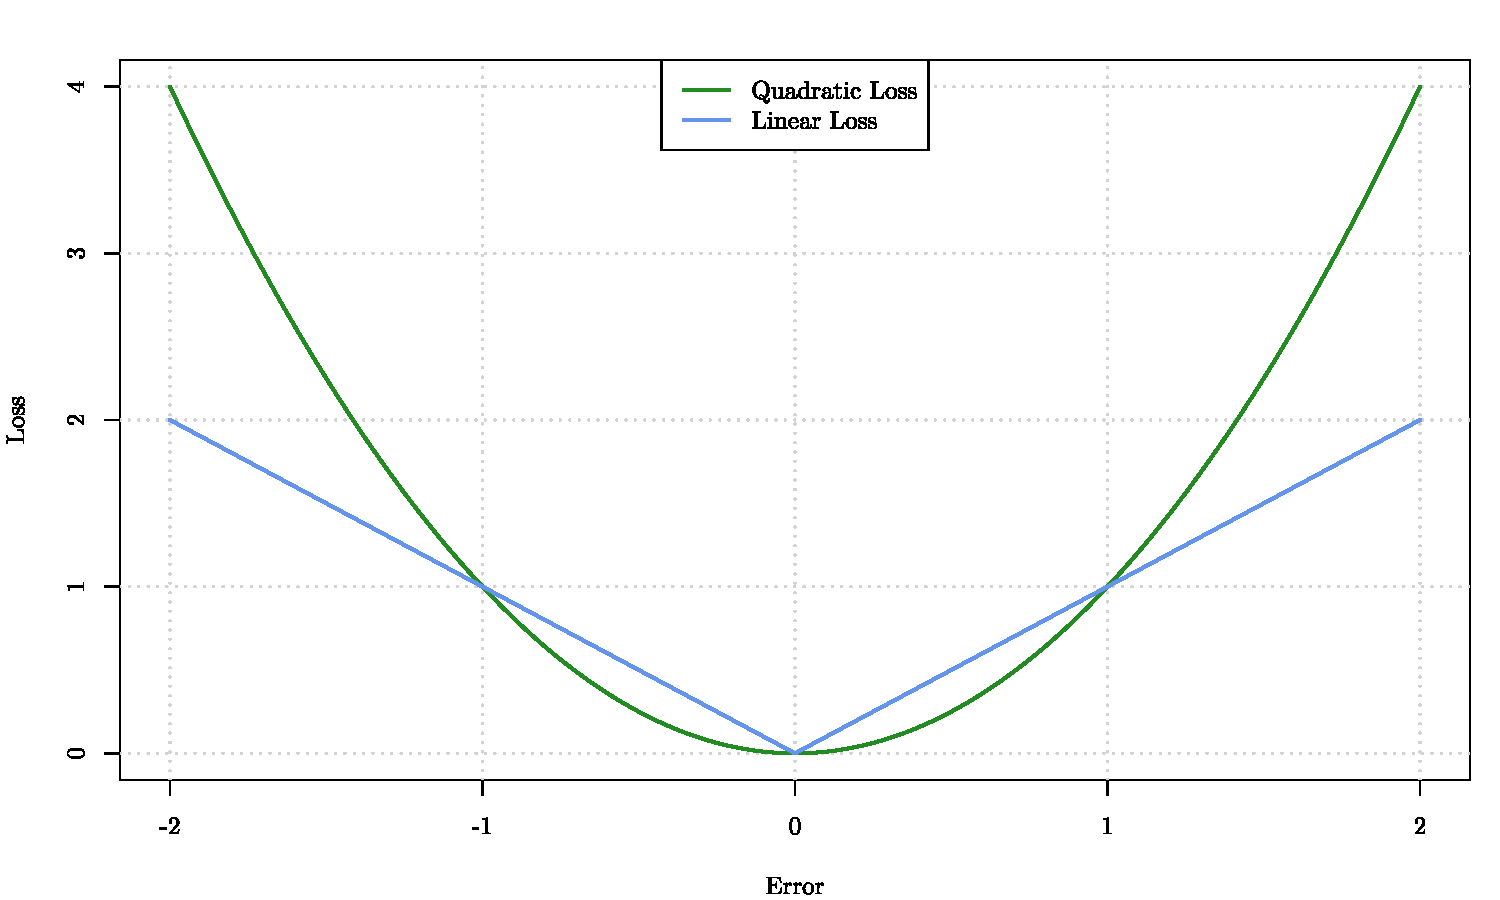
\includegraphics[width = 14	cm]{figures/Lossfun.pdf}
	\caption{Loss Functions}\label{fig:lossfun}
\end{figure}
\subsection{Prediction}\label{subsec:pred}
\subsubsection{Elastic Net}
\subsubsection{Random Forest}
\subsubsection{eXtreme Gradient Boosting}
\subsubsection{Performance Comparison}
\subsection{Unsupervised Colusion Detection}\label{subsec:col}
\section{Conclusion}\label{sec:con}
 
\newpage
\printbibliography
\end{document}